\section{Hardware Platform}

The ODROID-X2 developer platform \cite{hardkernelodroidx2} is used as a
reference hardware for all experiments in this thesis. An image of the platform
is shown in \autoref{fig:odroidx2}. Its core voltage is easily accessible on an
attached daughter board right beneath the heat sink, making it easy to conduct
power measurements. The board is equipped with a Samsung Exynos 4412 ``Prime'',
a modern System-on-Chip featuring four ARM Cortex-A9 CPU cores, Mali-400 GPU and
2GB of on-chip DRAM. The Cortex-A9 is one of ARM's mid-to-high-range application
processors. It features an out-of-order dual-issue speculative RISC core, and it
is clearly designed with emphasis on energy efficiency. This processor is
primarily found in low-powered embedded devices with some performance demands,
typically smartphones and tablets.

\begin{figure}
    \centering
    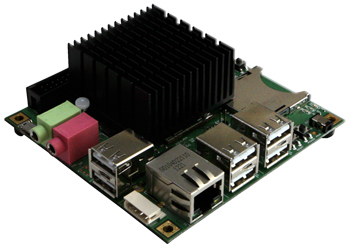
\includegraphics[width=0.7\textwidth]{figs/odroid.jpg}
    \caption{Image of the Hardkernel ODROID-X2 from the Hardkernel ODROID-X2 product page \cite{hardkernelodroidx2}}
    \label{fig:odroidx2}
\end{figure}

\begin{table}
    \centering
    \begin{tabular}{|c|c|}
        \hline
        Component      & Spesification\\
        \hline
        Manufacturer   & Hardkernel \\
        Platform       & ODROID-X2 \\
        SoC            & Samsung Exynos 4412 ``Prime'' \\
        CPU Core       & ARM Cortex-A9 \\
        Number of Cores& 4 \\
        Clock Frequency& 1.7GHz \\
        Core Voltage   & 1.3V \\
        L1             & Dual 32KB \\
        L2             & 1MB \\
        Main memory    & 2GB LP-DDR2 880MHz \\
        \hline
    \end{tabular}
    \caption{Hardware specifications ODROID-X2}
    \label{tab:hwspecx2}
\end{table}

After the decode stage, an out-of-order multi-issue module with speculation can
schedule two arithmetic operations, in which one can be a multiply (the
processor has only one hardware multiply unit). It also features a multiplexed lane
for address operations and floating point operations (the \emph{NEON} FPU). The
Cortex-A9 is often used as 1-4 cores \cite{armsite}, where the implementation
used on the Exynos 4412 is a 4-core variant \cite{somesite}. In this experiment,
3 of the cores are disabled to ease both the measurement and the simulation
process.

To achieve good simulation correctness, a high level of architectural knowledge
is crucial. Despite that most proprietary architectures have a lot of details
that remain undisclosed to the public, much information is still available.
Different sources have been used to find properties needed by the simulator,
some details regarding the OoO cores can be read about in
\cite{blem2013detailed}.
